\section{Data and Validation setup}

\begin{frame}{Data}
   
75 stock data from 2015 up to 2025 organized in 3 sectors (tech, healthcare, industrial)\\

   \vspace{5mm}
   
\begin{table}[H]
\centering
\resizebox{10cm}{!}{
\begin{tabular}{ccc}
\hline
\textbf{Technical} & \textbf{Economics} & \textbf{Others}\\
\hline
realized\_vol & gdp & sector\_sentiment \\
realized\_vol\_sma\_5 & cpi & economics\_sentiment \\
realized\_vol\_sma\_22 & ip & vix\_price \\
rv\_max\_5d & expected\_inflation & gprd \\
rv\_vol\_5d & term\_spread & is\_endofweek \\
rv\_max\_22d & default\_return & is\_startofweek \\
rv\_vol\_22d & usd-eur & weekend\_counter \\
vol\_regime & gold\_price & MACD\_signal \\
volume & crude\_price & MACD\_histogram \\
on\_balance\_volume & & MACD \\
relative\_volume & & \\
log\_return & & \\
\hline
\end{tabular}}
\end{table}

\end{frame}




\begin{frame}{Validation pipeline}
    The validation pipeline is used to statistically validate models performances, choose optimal hyperparameter settings and 
    assess if the proposed architecture actually beats benchmark models.\\

    \begin{figure} [H]
    \centering
    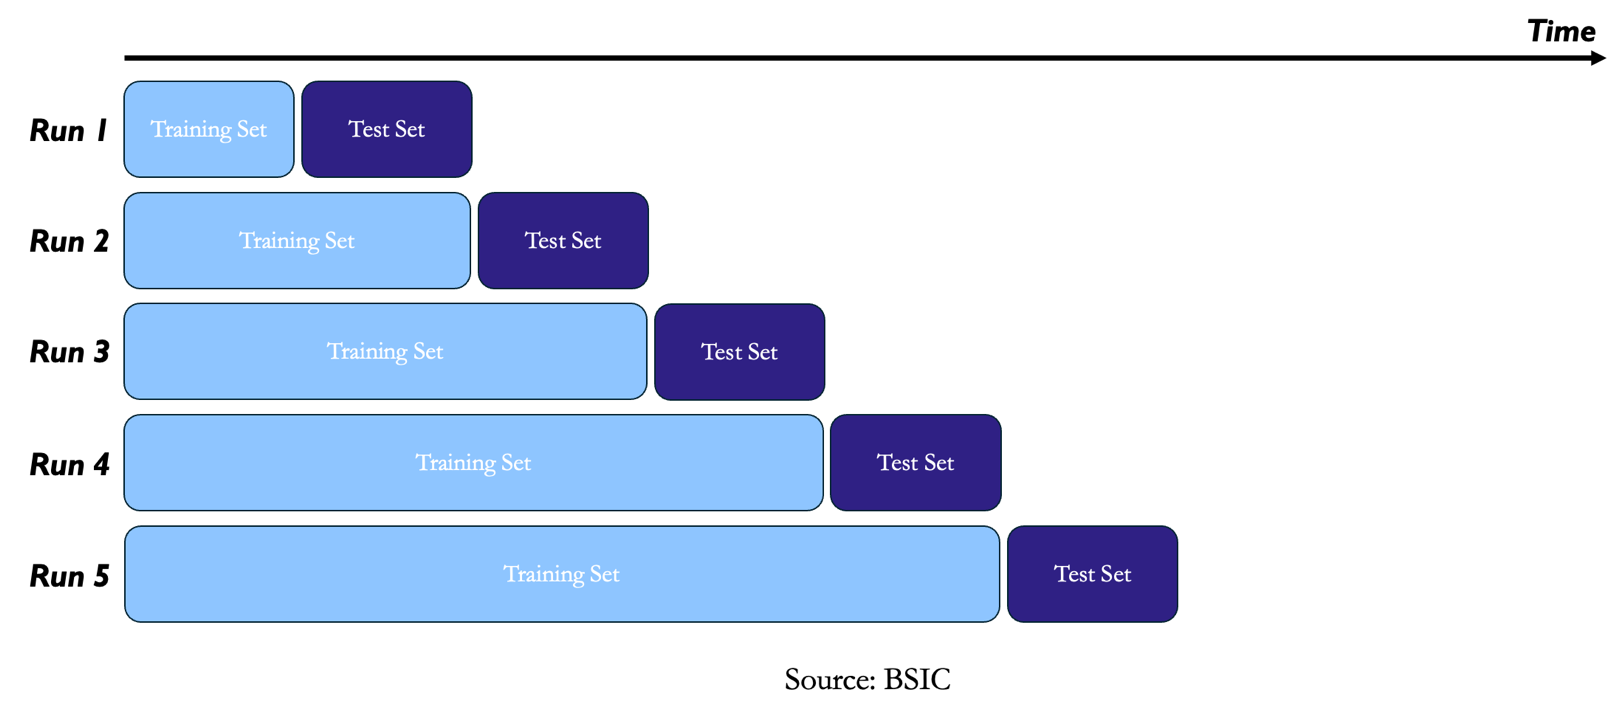
\includegraphics[scale=0.55]{images/walk-forward.png}
    \end{figure}


    The Purged cross-validation (or Walk forward) procedure is adopted using 
    3 folds and an embargo parameter consistent with the 22 days.

    
\end{frame}


\begin{frame}{Data processing}
For each training fold inside the walk forward procedure the following processes run

    \begin{itemize}
        \item log-transformation of skewed features
        \item Fractional differentiations allowing stationarity while preserving memory
        \item Feature selection through Boruta algorithm
        \item Data standardization 
        \item Optuna Hyperparameter tuning
    \end{itemize} 

The following error metrics are then computed on validation fold:
\begin{itemize}
    \item MSE
    \item RMSE
    \item MAE
    \item MAPE
    \item SMAPE
\end{itemize}

    
\end{frame}


\begin{frame}{Statistical Tests}
    To statistically define if the proposed model provides better forecasting performances with respect to 
rival models a 2 stage procedure is adopted.\\

\vspace{5mm}

\textit{Friedman Test}:
\begin{itemize}
    \item non-parametric test 
    \item $H0:$ all the $j$ competing models perform equivalently
    \item for each dataset the $j$ models are ranked for each error metric
    \item The average rank $R_j$ over the datasets is computed and the test statistic is built $\chi_F^{2}$ 
\end{itemize}


\textit{Nemenyi post-hoc test}:
\begin{itemize}
    \item If Friendman null hypothesis is rejected then the Nemenyi test is computed
    \item It determines whether the observed difference in $R_j$ between any two models is statistically significant
    \item Difference $|R_i -R_J|$ is compared to a Critical Difference value given a critical value $q_\alpha$.
\end{itemize}




\end{frame}
